\chapter{Overview on device-independent key distribution}

\section{Device-independent quantum key distribution}

As recent advances in quantum computing threaten the security of our current encryption algorithm~\cite{Gouzien2021,Gouzien2023}, more-than-ever is the need for stronger cryptographic protocol. 
One candidate is \acrfull{QKD}, allowing two parties to share a secret key, in a provably secure way, by using quantum properties.
\acrshort{QKD} can be formulated as an entanglement-based protocol in which Alice and Bob generate a key from the outcome of specific measurements performed on a shared entangled state they receive~\cite{Ekert1991}. 
The security of this protocol relies on the following assumptions
\begin{itemize}
	\item 1. The devices used to generate the key behave according to quantum theory,
	\item 2. There is no information leakage out of Alice and Bob systems, e.g. Alice and Bob are each in a hermetic laboratory,
	\item 3. Alice and Bob have access to random numbers,
	\item 4. The quantum devices used to perform measurements is perfectly calibrated and behave predictably.
\end{itemize}

Trust in cryptography can not go further than trust in the assumptions we make on our cryptographic protocols. 
In this scope, it is highly desirable to remove the assumption on the quantum devices used to perform measurements.
Indeed, the devices or the apparatus composing these devices can be bloated by a third party producer.
A famous example of such interference on classical system is the cryptographic devices sold by Crypto AG which were bugged by the Central Intelligence Agency~\cite{Miller2020}.
However, even considering an honest manufacturer, the quantum devices implementing QKD are hard to build and will always contain noises and losses.
These perfections have been exploited to successfully attack QKD protocols~\cite{Fung2007,Lydersen2010,Gerhardt2011,Weier2011}.

\medbreak

Introducing \acrfull{DIQKD}, a family of more secure quantum key distribution protocols in which the assumption on the inner working of the quantum devices is dropped.
Intuitively, these protocols could use a similar approach to self-testing, in which Bell games would asses the presence of non-locality from classical outputs of measurements on a shared system, which would then be converting into a security proof on the distributed key.
However, this approach leads to performance far from practical applications~\cite{Fu2018,Kundu2022}.
Hence, for better efficiency, the security proof of most protocols is directly based on the observed correlations and not from a self-test.
Security proofs are briefly presented in Chap.~\ref{chap:entropybound}.


\section{A DIQKD protocol}

Alice and Bob wants to share a cryptographic key, unknown to an eavesdropper, Eve, which has access to unlimited physical and computational resources.
Both parties are each in a closed labs such that no information is leaked, and each have access to a trusted source of randomness.
These labs are interconnected by a quantum channel as well as by an authenticated classical channel.
Note that the classical channel is public, all the information transmitted over it is openly disclosed.

In her lab, Alice has two measurements $\hat{A}_x$, with $x\in \{0,1\}$.
In his lab, Bob has three measurements $\hat{B}_y$, with $y \in \{0,1,2\}$.
The outcomes of the measurements $\hat{A}_0,\hat{A}_1,\hat{B}_0$ and $\hat{B}_1$ are used to guarantee the secrecy of the generated key.
The extra measurement $\hat{B}_2$ is chosen so that it correlates with $\hat{A}_0$.
If the outcomes of all measurements can be non-binary, Alice and Bob can always locally process their outcomes to binary values $\{\pm1\}$.

In the following, we make no assumption on the quantum channel and the measurements, i.e. Eve is considered to have full control over the quantum channel and can have bugged the measurement devices beforehand.
A setup to perform DIQKD is depicted in \reffig{DIQKD_setup}.

\medbreak

With this setup, a typical DIQKD protocol has the following steps
\begin{enumerate}
		\item Preparation: Alice and Bob agree on which protocol rounds to use to test the device, i.e. to verify if the observed correlations fulfill some requirements or to abort the protocol otherwise. These rounds are referred as \textit{test rounds}, while the other rounds are \textit{generation rounds}.
		\item Measurements: For each rounds, a source generate and distribute a shared quantum state $\ket{\psi_{ABE}} \in \Hil_a \otimes \Hil_B \otimes \Hil_E$ to Alice and Bob over the quantum channel. Alice randomly picks an input $x\in\{0,1\}$ and preform the corresponding measurement $\hat{A}_x$. Bob measures with either $\hat{B}_0$ or $\hat{B}_1$, chosen randomly, in case of a test round, or with $\hat{B}_2$ for a generation round. Alice records the obtained outcome in a string
			$\mathbf{A}$. Similarly Bob fill a string $\mathbf{B}$ from his outcome. At the end of the measurement rounds, Alice and Bob share the string of their input choices, $\mathbf{X}$ and $\mathbf{Y}$, respectively.
		\item Sifting: Alice and Bob may erase the outcomes of some generation rounds. This is particularly relevant for basis choice leading to poorly correlated outcomes. In the setup we consider, this is all generation rounds in which Alice measured $\hat{A}_1$. 	
	\item Error correction: Alice and Bob communicate publicly some bits of their outcomes strings. This allow Bob to either reconstruct a string $\mathbf{A'}=\mathbf{A}$ or abort the protocol.
	\item Parameter estimation: From $\mathbf{A'},\mathbf{B},\mathbf{X}$ and $\mathbf{Y}$ Bob can compute the correlations $p(ab|xy)$. If these correlations fail to satisfy some requirements, e.g. a given CHSH score, the protocol abort. 
	\item Privacy amplification: Alice and Bob run a privacy amplification amplification using some of the bits of $\mathbf{A},\mathbf{B}$, to yield the final keys.
\end{enumerate}

Some extra steps can be included to further hence the performance of DIQKD protocols.
Notably, following insights on QKD, Alice can add noise by shifting the outcomes of $\hat{A}_0$ with a probability fixed before the protocol starts~\cite{Ho2020}. 

\begin{figure}
	\begin{center}
		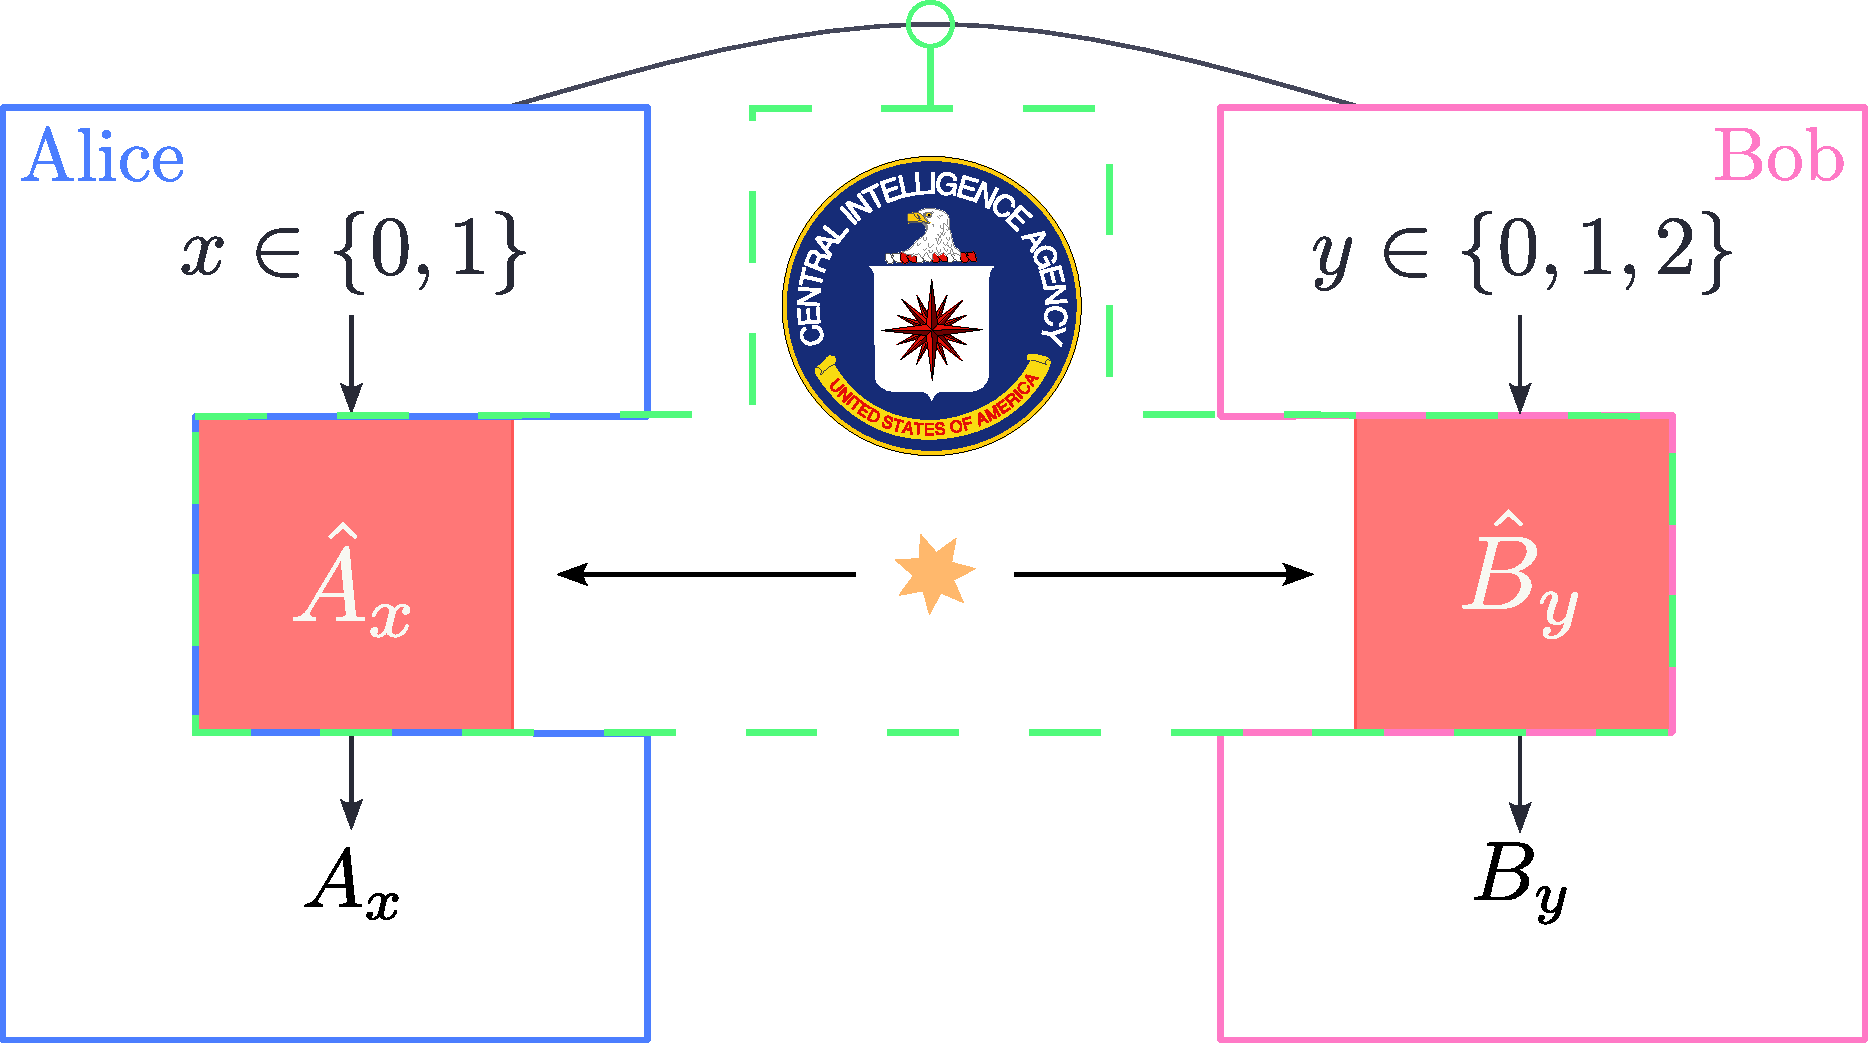
\includegraphics[width=0.95\textwidth]{chapters/deviceindependent/img/setup.pdf}
	\end{center}
	\caption{DIQKD Setup. Alice's lab (delimited by the blue line) and Bob's lab (delimited by the pink line) are linked by a classical channel of communication (gray cruved line), and by a quantum channel (green dashed rectangle). A source (yellow star) generate a state with one part send to Alice while the other is send to Bob. Alice select an input $x$, to perform the measurement $\hat{A}_x$ and obtain the outcome $A_x$. Similarly Bob chose an input $y$, to measure with respect to $\hat{B}_y$ and obtain $B_y$.
	Eve, represented by the CIA logo, has full access to the quantum channel, and may have bloated the measurement devices. }
	\label{fig:DIQKD_setup}
\end{figure}

